\documentclass{article}
\textheight24cm\textwidth16cm\topmargin-1cm
\oddsidemargin0cm\evensidemargin0cm

\usepackage{amsmath,amssymb}
% \usepackage[dvipdfmx]{graphicx}
\usepackage{graphicx}
\usepackage{subfigure}

\usepackage{url}
\usepackage{bm}
\usepackage{setspace} 

% \usepackage{algorithmic}
% \usepackage{algorithm}

\newtheorem{thm}{Theorem}
\newtheorem{dfn}[thm]{Definition}
\newtheorem{lem}[thm]{Lemma}
\newtheorem{prop}[thm]{Proposition}
\newtheorem{cor}[thm]{Corollary}
\newcommand{\proof}{\noindent Proof.\ \ }
% \renewcommand{\algorithmiccomment}[1]{// #1}


%\pagestyle{empty}


\begin{document}

% \baselineskip 6.5mm

\vspace*{1.0cm}
{\LARGE \bf Supplementary material}
\vspace*{0.25cm}


\section*{Derivation of EM algorithm}


The complete log-likelihood including missing data $\{ \bm{z}_i \}$ for the proposed model is
\begin{equation*}
\sum_{i = 1}^I \sum_{j=1}^J \sum_{k=1}^K I(z_{i,j} = k) \Bigl( \sum_{l = 1}^L \log f_{k, l, x_{i,j,l}} + \log q_{i,k} \Bigr).
\end{equation*}
Here, we introduce the variable for conditional probability for $z_{i,j}$ given the parameters and the mutation features $\bm{x}_{i,j}$,
\begin{equation*}
\theta_{i,k, \bm{m}} = \Pr \bigl( z_{i,j} = k \big| \bm{x}_{i, j} = \bm{m}, \{ \bm{f}_{k, l} \}, \{  \bm{q}_i \} \bigr)
\end{equation*}
Note that this conditional probability just depends on the value of mutation feature $\bm{m} = (m_1, \cdots, m_L)$, not on the index $j$.
Then, the expected complete log-likelihood augmented by Lagrange multipliers is calculated as
\begin{equation*}
\sum_{i=1}^I \sum_{\bm{m}} g_{i, \bm{m} } \sum_{k=1}^K \theta_{i, k, \bm{m}}   \Bigl( \sum_{l = 1}^L \log f_{k, l, m_l} + \log q_{i,k} \Bigr)
+ \sum_{k=1}^K \sum_{l=1}^L \tau_{k,l} \bigl( 1 - \sum_{p=1}^{M_l} f_{k,l,p} \bigr)
+ \sum_{i=1}^I \rho_i \bigl( 1 - \sum_{k=1}^K q_{i,k} \bigr).
\end{equation*}
Differentiating it leads to following stationary equations: 
\begin{align*}
\sum_{i=1}^I \sum_{\bm{m}: m_l = p} g_{i, \bm{m}} \theta_{i,k,\bm{m}} - \tau_{k,l} f_{k,l,p} & = 0,\ (p=1, \cdots, M_l, k=1, \cdots, K,\ l=1, \cdots, L)., \\
\sum_{\bm{m}} g_{i,\bm{m}} \theta_{i,k,\bm{m}} - \rho_i q_{i, k} & = 0,\ (k = 1, \cdots, K, i = 1, \cdots, I).
\end{align*}
Then, by eliminating Lagrange multipliers, updating rules can be obtained.



\section*{Relationship with nonnegative matrix factorization}

First, for ease of explanation, let assume that the full representation'' representation ($L = 1$) is used.
Suppose that each $\bm{m}$ has unique appropriate index from 1 to  $| \bm{M} | = \prod_{l=1}^L M_l$ (the number of possible mutation patterns),
so that $\bm{m}$ can be indices of matrices.

Let $G = \{ g_{i, \bm{m}} \}$ denote the $I \times | \bm{M} | $ matrix, 
where $g_{i, \bm{m}}$ is the number of mutations whose mutation patters are equal to $\bm{m}$ in the $i$-th cancer genome.
Nonnegative matrix factorization aims to find low rank decomposition, 
$G \sim \tilde{Q} F$,
where $\tilde{Q} = \{ \tilde{q}_{i,k} \}$ and $F = \{ f_{k, \bm{m}} \}$ are nonnegative matrix, 
and row vectors of $F$ are often restricted to be sum to one. 
We used the notation $\tilde{Q}$ instead of $Q$
to represent that the row vectors of $\tilde{Q}$ are not normalized to sum to one in general.

For solving NMF, 
the previous study \cite{pmid23318258} used the following updating rule \cite{Lee00algorithmsfor}:
\begin{equation*}
f_{k,m} \gets f_{k,m} \frac{ ( \tilde{Q}^T G)_{k,m} }{ ( \tilde{Q}^T \tilde{Q} F  )_{k,m} },\  \
\tilde{q}_{i,k} \gets \tilde{q}_{i,k}  \frac{ (G F^T)_{i,k} }{ ( \tilde{Q} F F^T )_{i,k} },
\end{equation*}
that reduces the {\it Euclidean distance} $|| G - \tilde{Q} F ||$. 
Therefore, the optimization problem for the existing approach is
\begin{equation}
\begin{aligned}
& \text{minimize}
& & ||G - \tilde{Q} F || \\
& \text{subject to}
& & \sum_{ \bm{m} } f_{k, \bm{m}} =  1, \; k = 1, \cdots, K \\ &
& & f_{k, \bm{m}} \geq 0, \; k = 1, \cdots, K,\ \bm{m} \in M \\ & 
& & \tilde{q}_{i, k} \geq 0, \; i = 1, \cdots, I,\ k = 1, \cdots, K.
\end{aligned}
\end{equation}

On the other hand, there is another type of updating rule \cite{Lee00algorithmsfor}:
\begin{equation*}
f_{k,m} \gets f_{k,m} \frac{ \sum_i \tilde{q}_{i,k} g_{i,m} / ( \tilde{Q} F)_{i,m} }{ \sum_i \tilde{q}_{i,k} },
\end{equation*}
\begin{equation*}
\tilde{q}_{i,k} \gets \tilde{q}_{i,k}  \frac{ \sum_m f_{k,m} g_{i,m} / ( \tilde{Q} F)_{i,m} }{ \sum_m f_{k,m} }.
\end{equation*}
that reduces the Kullback-Liebler Divergence:
\begin{equation*}
KL(G ||  \tilde{Q} F) = \sum_{i,m} \Bigl( g_{i,m} \log  \frac{ g_{i,m} }{ (\tilde{Q} F)_{i,m} } - g_{i,m} + ( \tilde{Q} f )_{i,m} \Bigr).
\end{equation*}

In general cases including the independent representation, 
there is restrictions $f_{k, \bm{m}} = \prod_l f_{k, l, m_l}$ by smaller set of parameters.
Let us consider the following optimization problem with the Kullback-Liebler Divergence and the restrictions on $F$:
\begin{equation}
\begin{aligned}
& \text{minimize}
& & KL(G ||  \tilde{Q} F) \\
& \text{subject to}
& & f_{k, \bm{m}} = \prod_l f_{k, l, m_l}, \; k = 1, \cdots, K,\ \bm{m} \in M \\ & 
& & f_{k, l, p} \geq 0, \; k = 1, \cdots, K,\ \bm{m} \in M \\ & 
& & \tilde{q}_{i, k} \geq 0, \; i = 1, \cdots, I,\ k = 1, \cdots, K.
\end{aligned}
\label{KL}
\end{equation}

In fact, this is equivalent to the proposed method, whose optimization problem can be written as:
\begin{equation}
\begin{aligned}
& \text{maximize}
& & L(Q, F | G) \bigl(= \sum_{i,m}  g_{i,m} \log (Q F)_{i,m} \bigr)  \\
& \text{subject to}
& & f_{k, \bm{m}} = \prod_l f_{k, l, m_l}, \; k = 1, \cdots, K,\ \bm{m} \in M \\ & 
& & f_{k, l, p} \geq 0, \; k = 1, \cdots, K,\ \bm{m} \in M \\ & 
& & \sum_k  q_{i, k} =  1, \; i = 1, \cdots, I \\ &
& & q_{i, k} \geq 0, \; i = 1, \cdots, I,\ k = 1, \cdots, K.
\end{aligned}
\label{likelihood}
\end{equation}

\begin{prop}
When $(Q, F) = (Q^*, F^*)$ is an optimal solution of the optimization problem (\ref{likelihood}), 
then $(\tilde{Q}, F) = (R^* Q^*, F^*)$ is an optimal solution of the optimization problem (\ref{KL}).
On the other hand, when $(\tilde{Q}, F) = (\tilde{Q}^*, F^*)$ is an optimal solution of the optimization problem (\ref{KL}),
then $(Q, F) = (R^{*-1} \tilde{Q}^*, F^*)$ is an optimal solution of the optimization problem (\ref{likelihood}),
where $R^* = \text{diag} (r_1^*, \cdots, r_I^*), r_i^* = \sum_{\bm{m}} g_{i,\bm{m}}, i = 1, \cdots, I$.
\end{prop}
\proof
This is because
\begin{equation*}
KL(G ||  \tilde{Q} F) = -  \sum_i \Bigl( ( \sum_{m} g_{i, m} ) \log \tilde{r}_i - \tilde{r}_i \Bigr)  - L(Q, F | G) + \text{(constant value)},
\end{equation*}
where $Q$ is row-normalized matrix for $\tilde{Q}$, $\tilde{r}_i = \sum_k q_{i, k}$ for each $i$, 
and $( \sum_{m} g_{i, m} ) \log \tilde{r}_i - \tilde{r}_i$ takes its maximum at $\tilde{r}_i = r_i^*$.
\hfill $\square$

% \bibliographystyle{natbib}
%\bibliographystyle{achemnat}
%\bibliographystyle{plainnat}
%\bibliographystyle{abbrv}
%\bibliographystyle{bioinformatics}
\bibliographystyle{plain}
\bibliography{document}



\clearpage

\begin{figure}
\centering
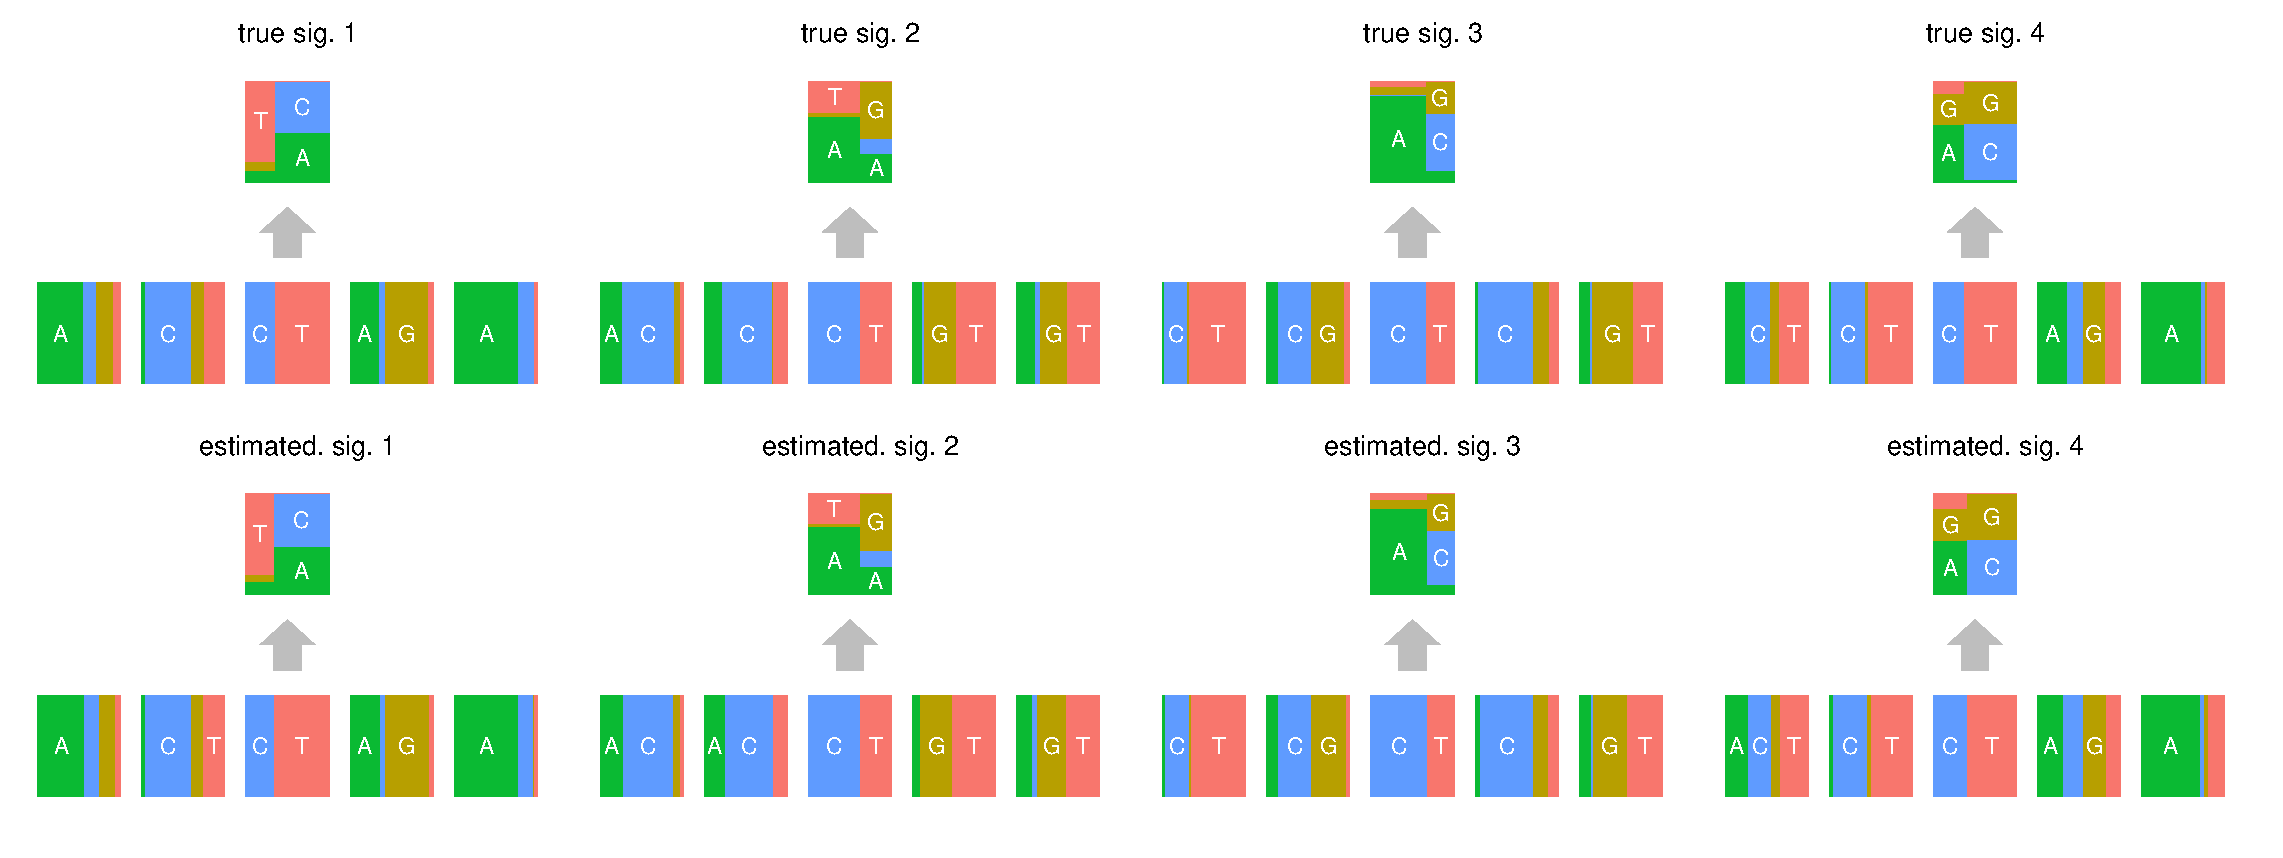
\includegraphics[width=15cm,height=5.5cm]{simulation_signature_example.eps}
\caption{}
\label{example_signature.pd}
\end{figure}


\clearpage

\begin{figure}
\centering
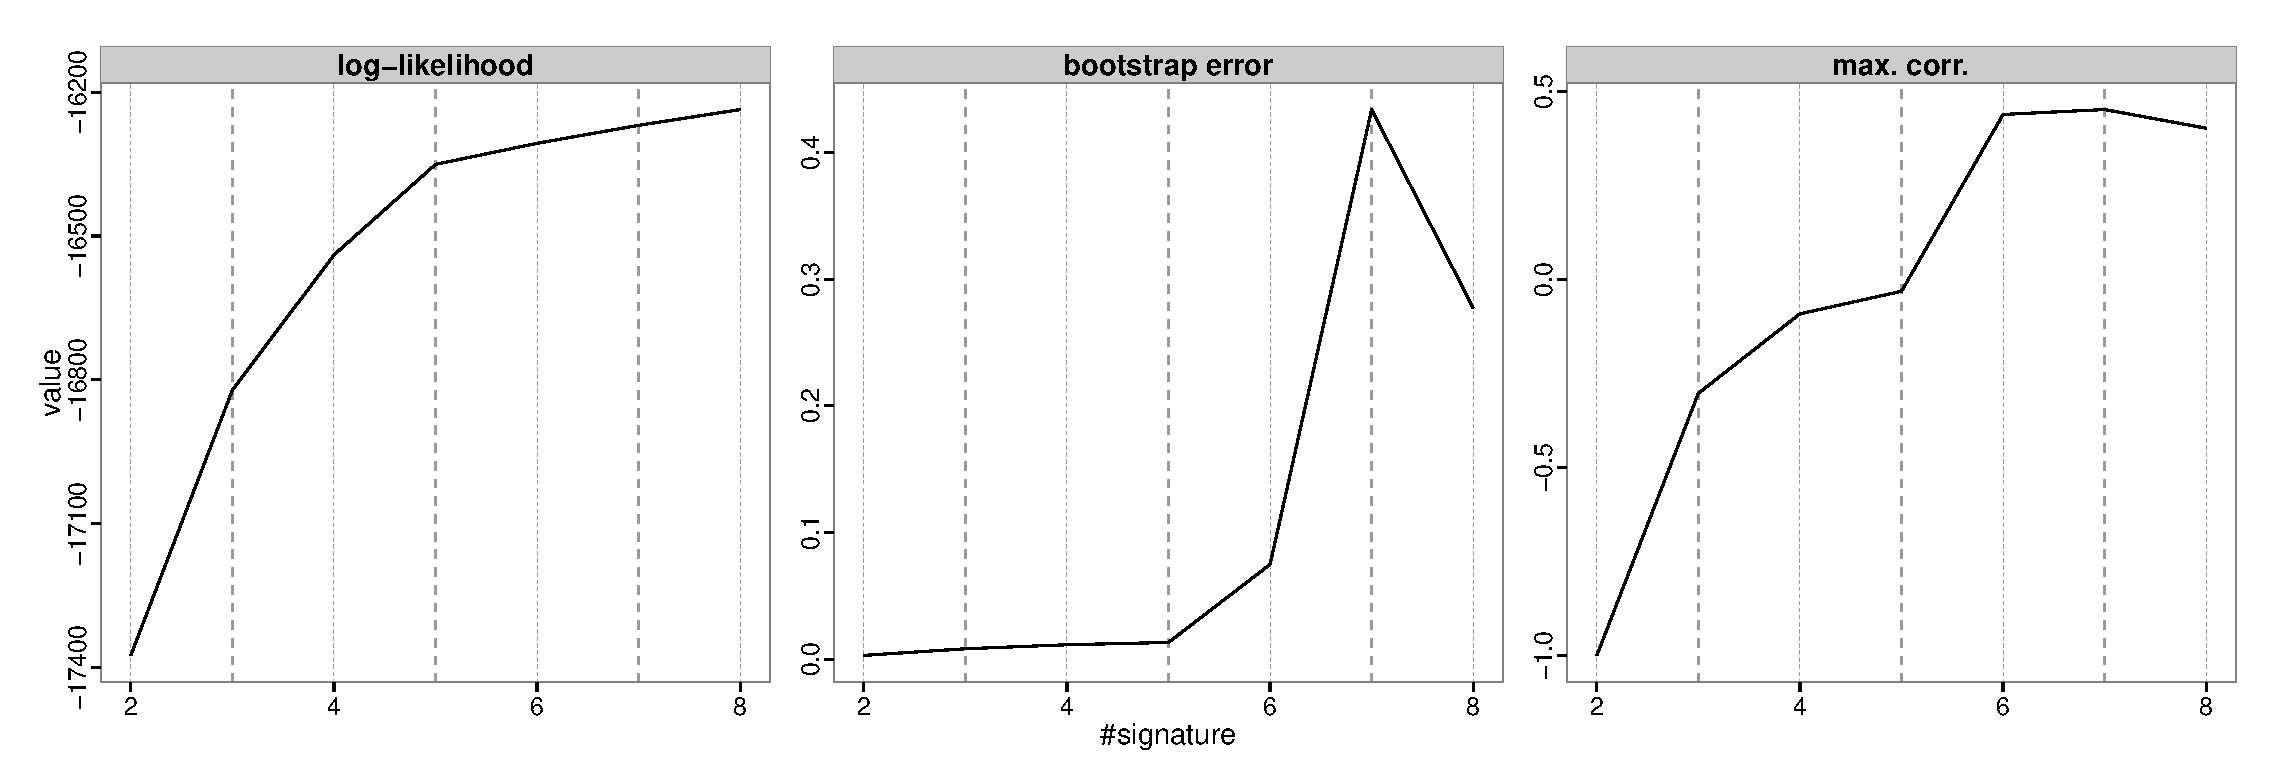
\includegraphics[width=15cm,height=5cm]{simulation_stat.eps}
\caption{}
\label{example_summary.pd}
\end{figure}

\clearpage


\begin{figure}
\centering

\subfigure[Estimated mutation signatures ($K = 2$)]{%
  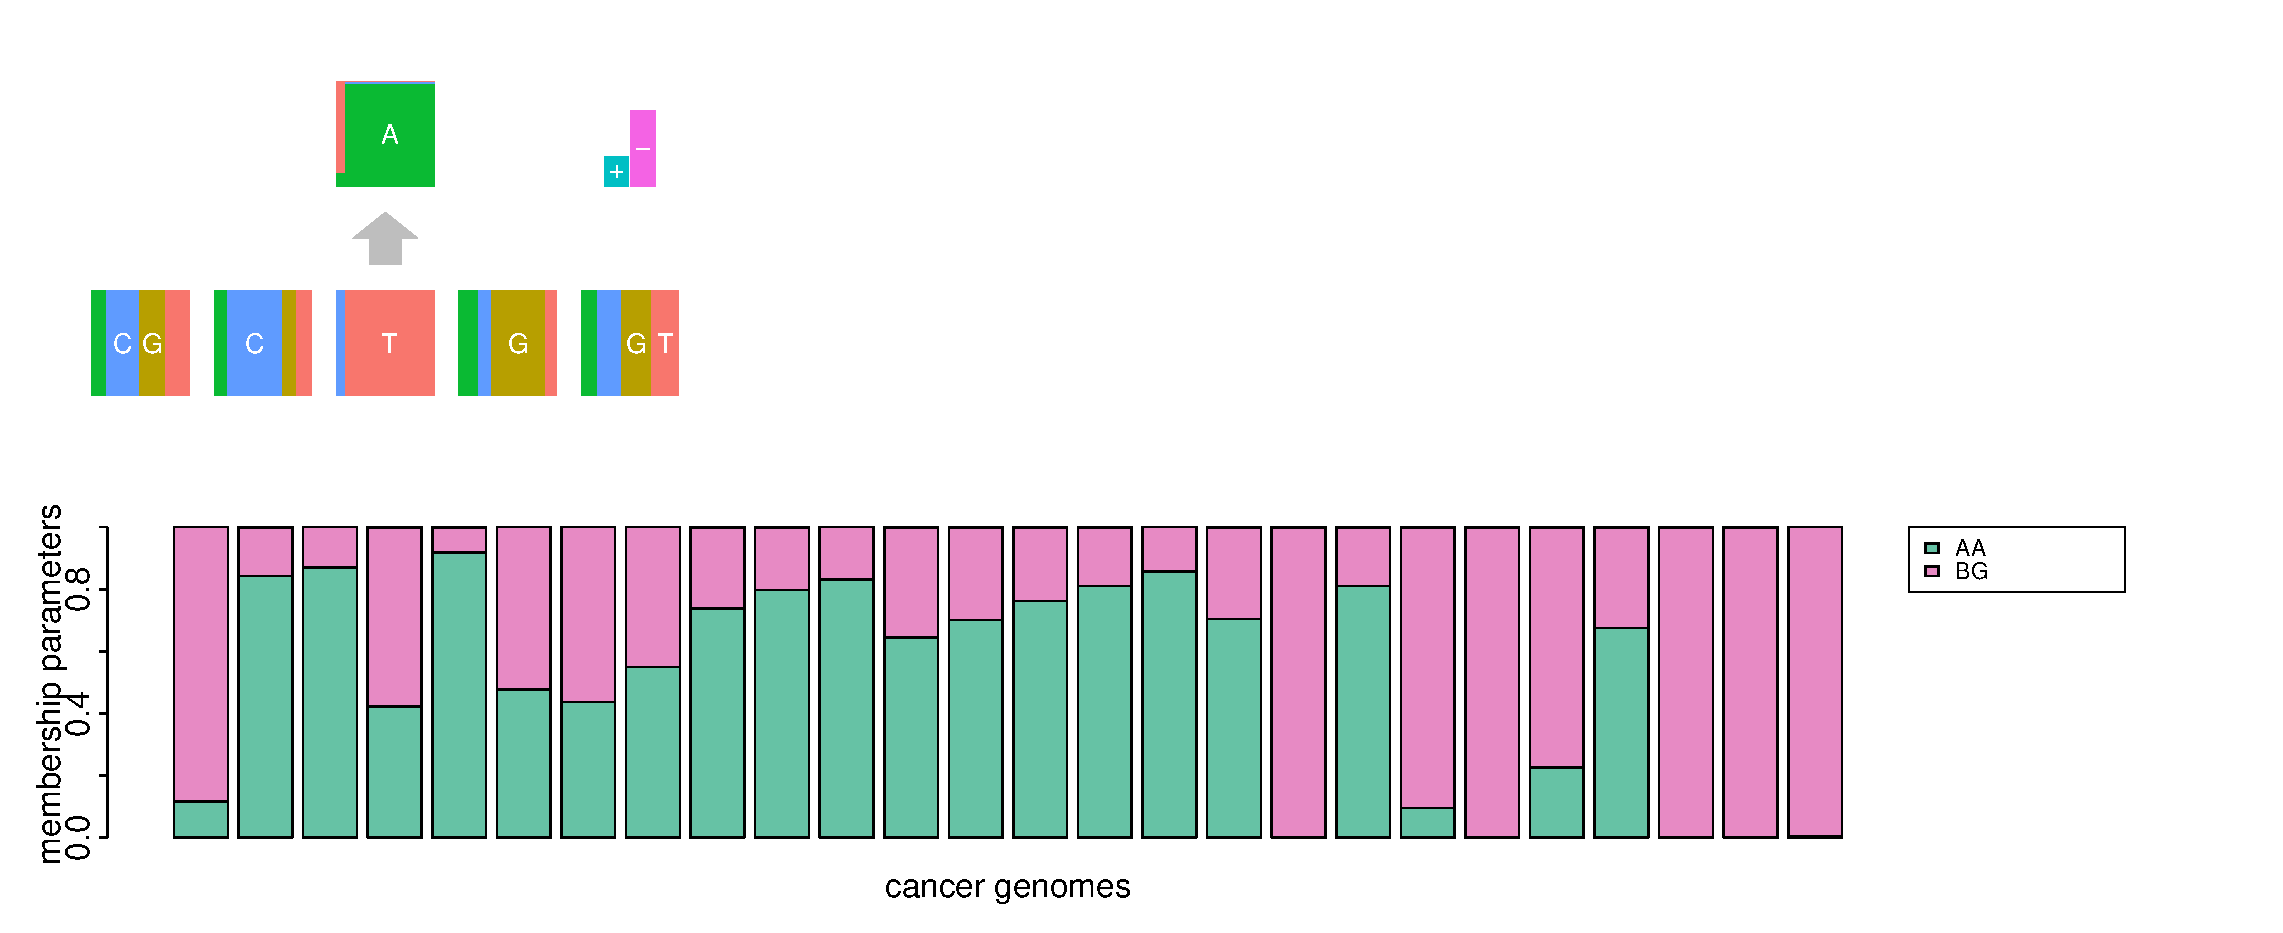
\includegraphics[height=6cm,width=15cm,clip]{UTUC_signature_K2.eps}
  \label{UTUC:sigK2_sig}}
  
  
\subfigure[Estimated mutation signatures ($K = 3$)]{%
  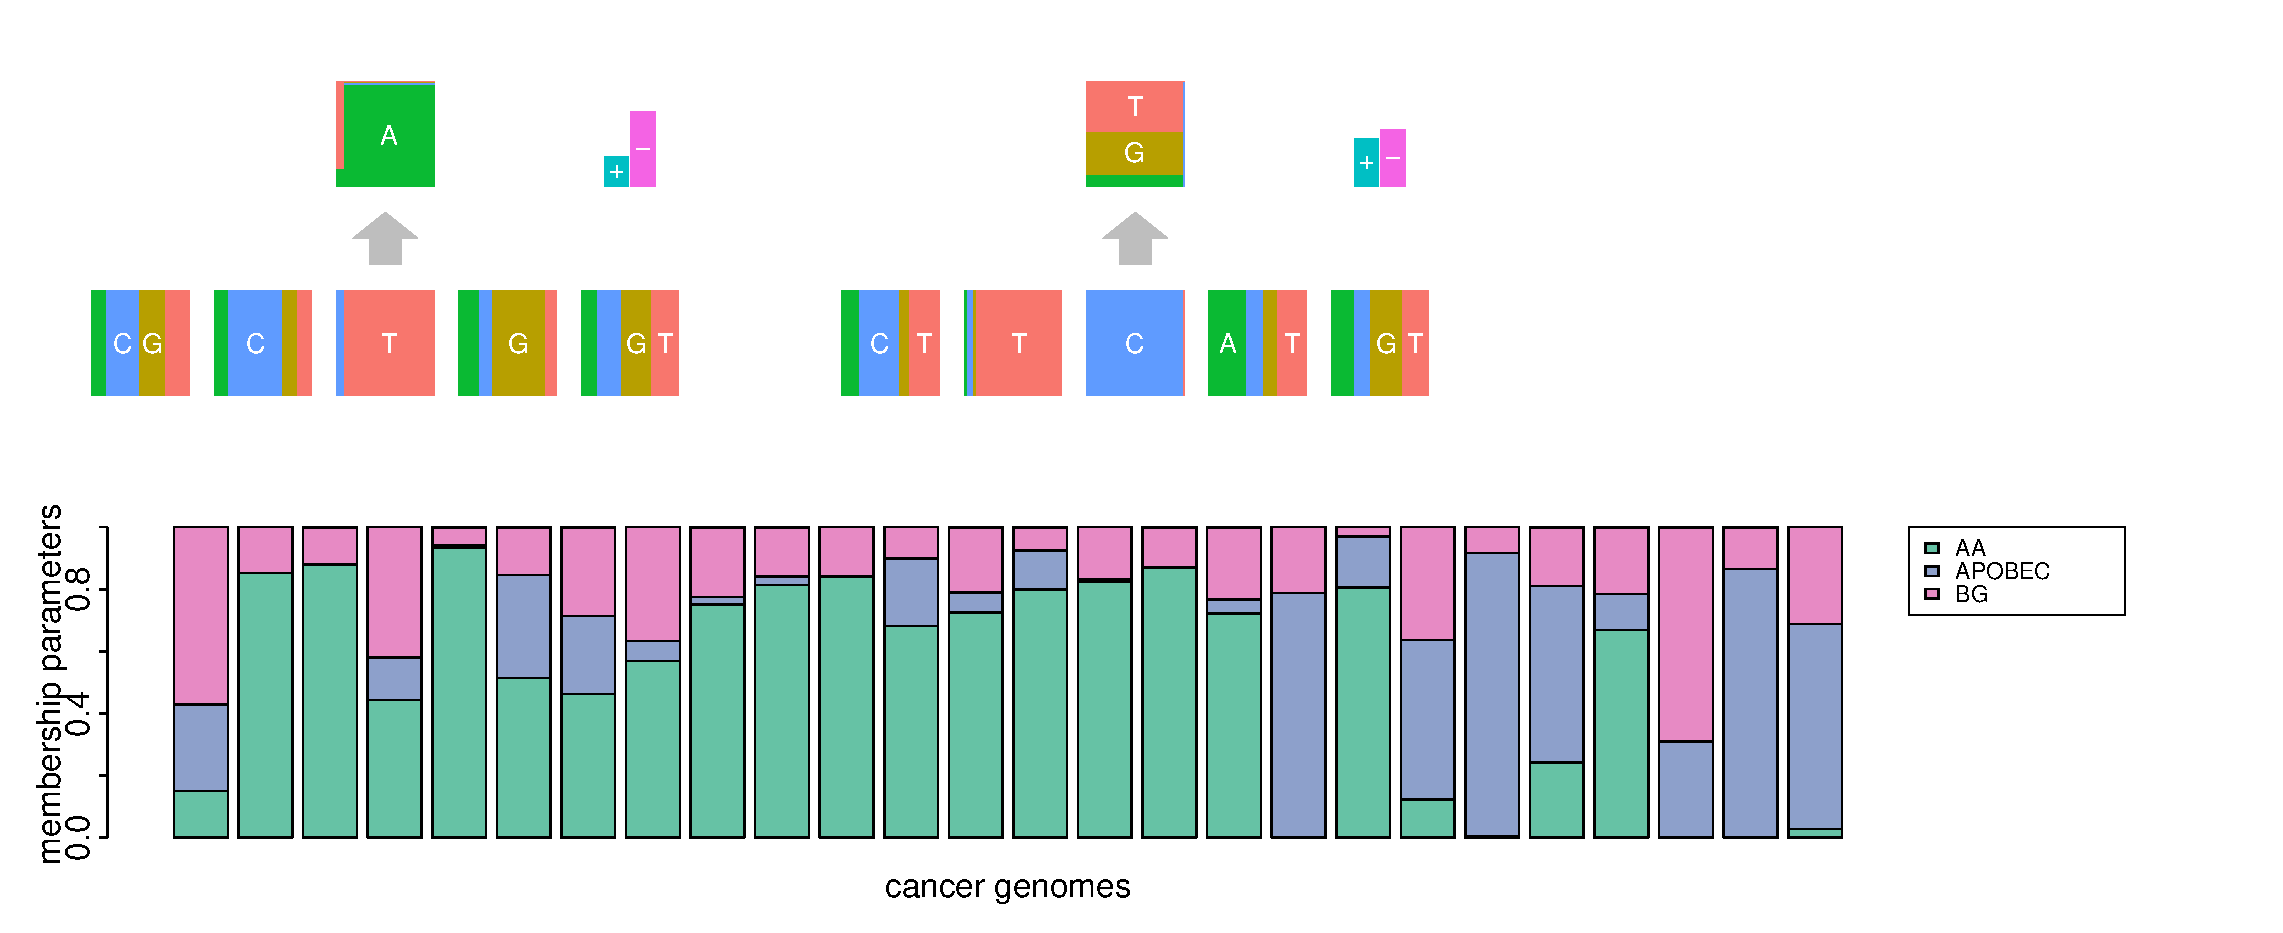
\includegraphics[height=6cm,width=15cm,clip]{UTUC_signature_K3.eps}
  \label{UTUC:sigK3_sig}}
  

\subfigure[Estimated mutation signatures ($K = 4$)]{%
  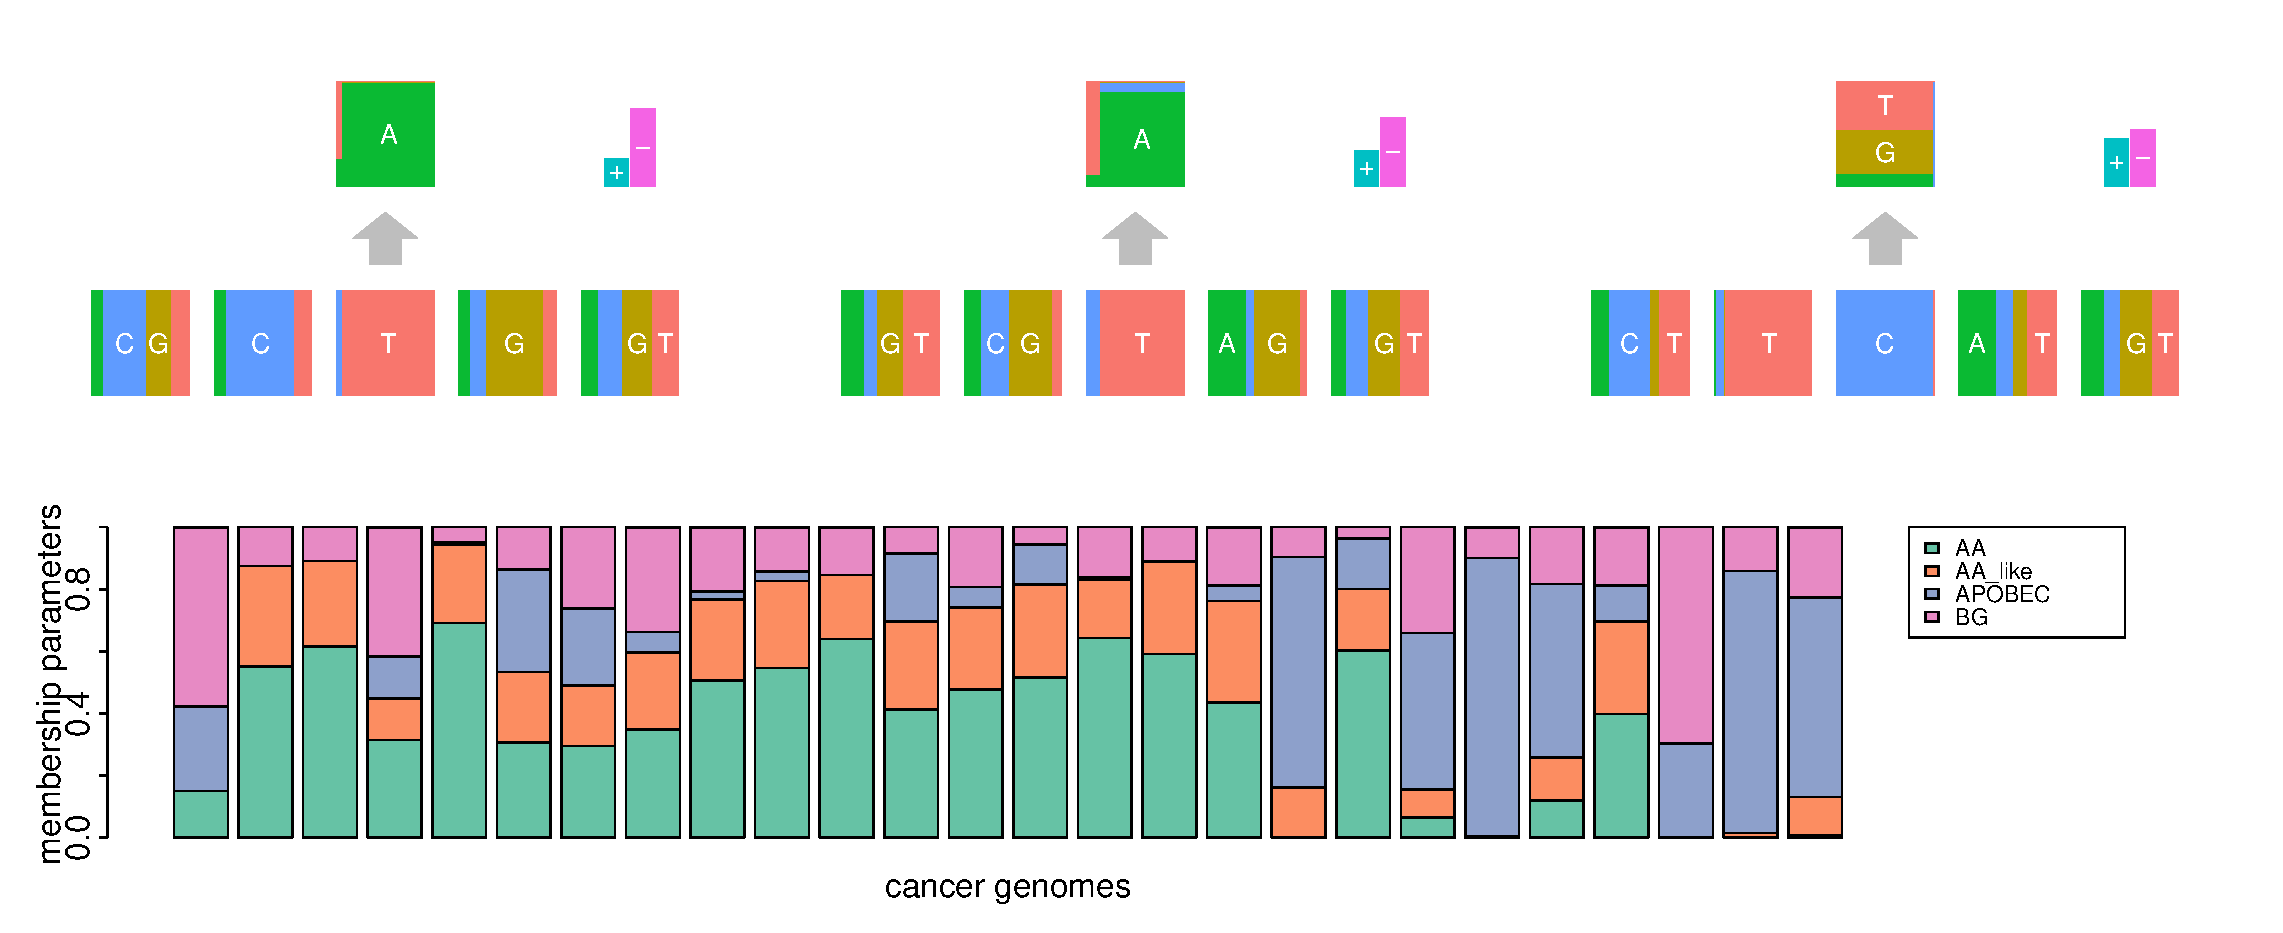
\includegraphics[height=6cm,width=15cm,clip]{UTUC_signature_K4.eps}
  \label{UTUC:sigK4_sig}}

  
\caption{The result of estimated mutation signatures and membership parameters for UTUC data 
when changing the number of mutation signatures ($K$).}
\label{UTUC_multiK}
\end{figure}

\clearpage

\begin{figure}
\centering
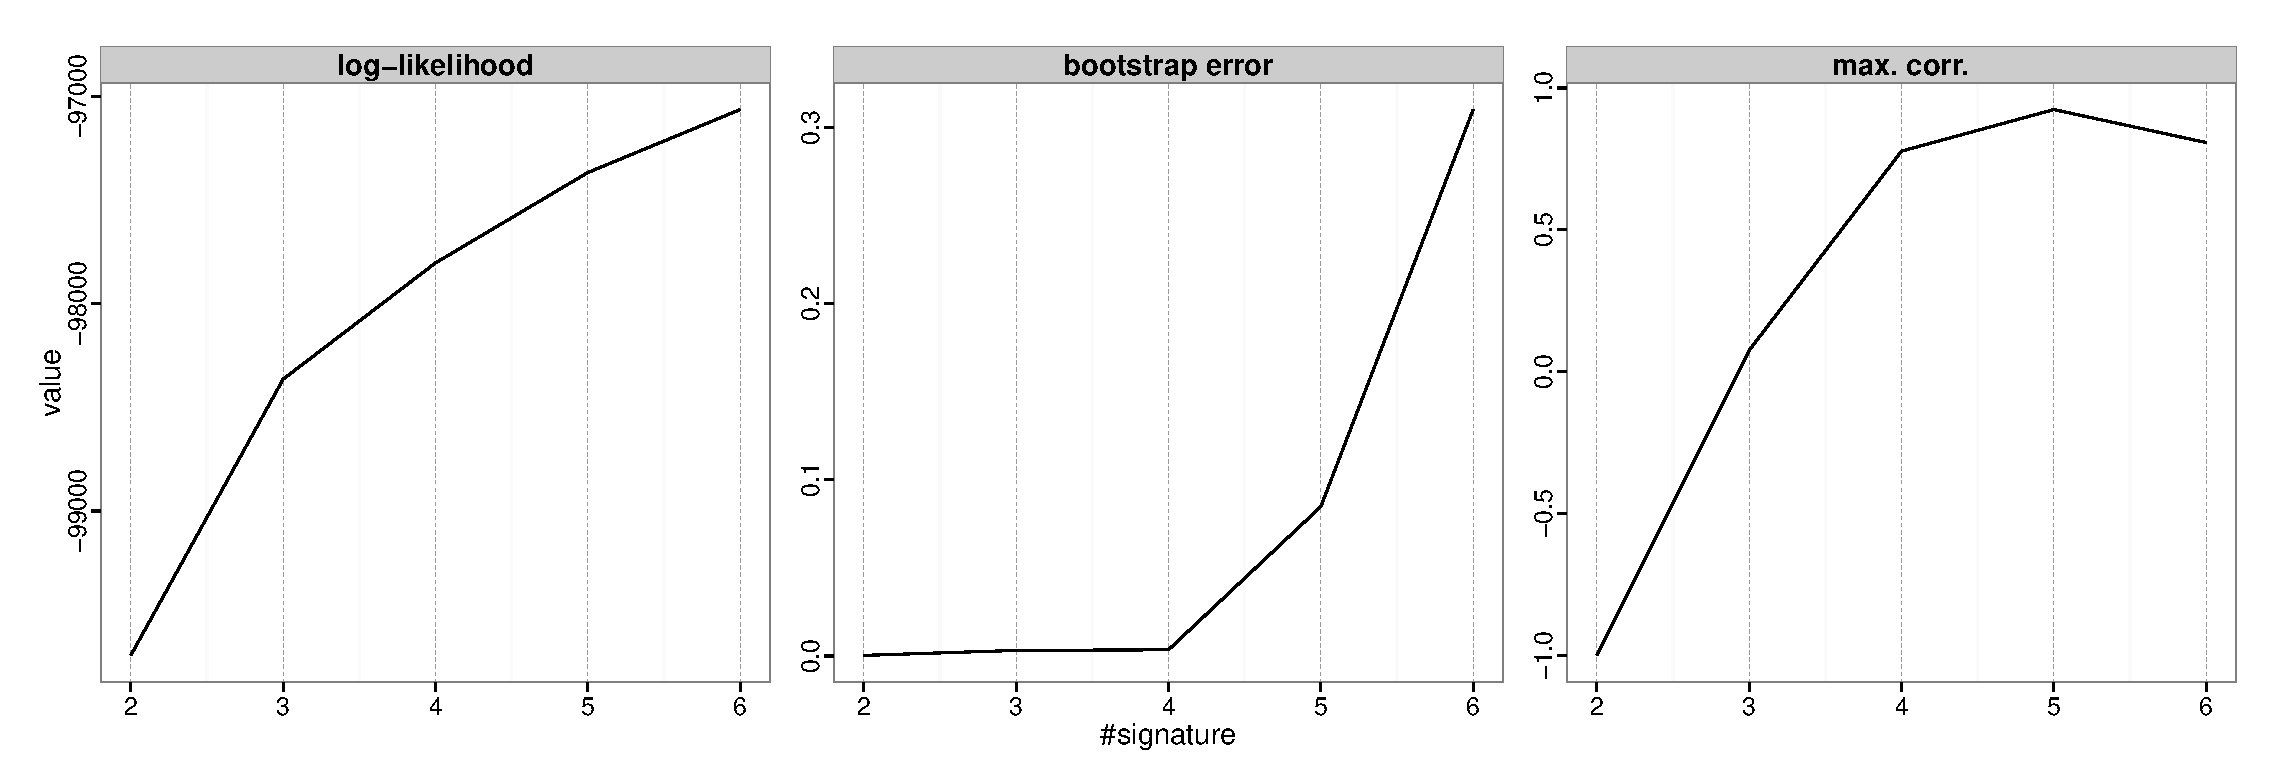
\includegraphics[width=15cm,height=5cm]{UTUC_stat.eps}
\caption{}
\label{example_summary.pd}
\end{figure}

\clearpage

\begin{figure}
\centering
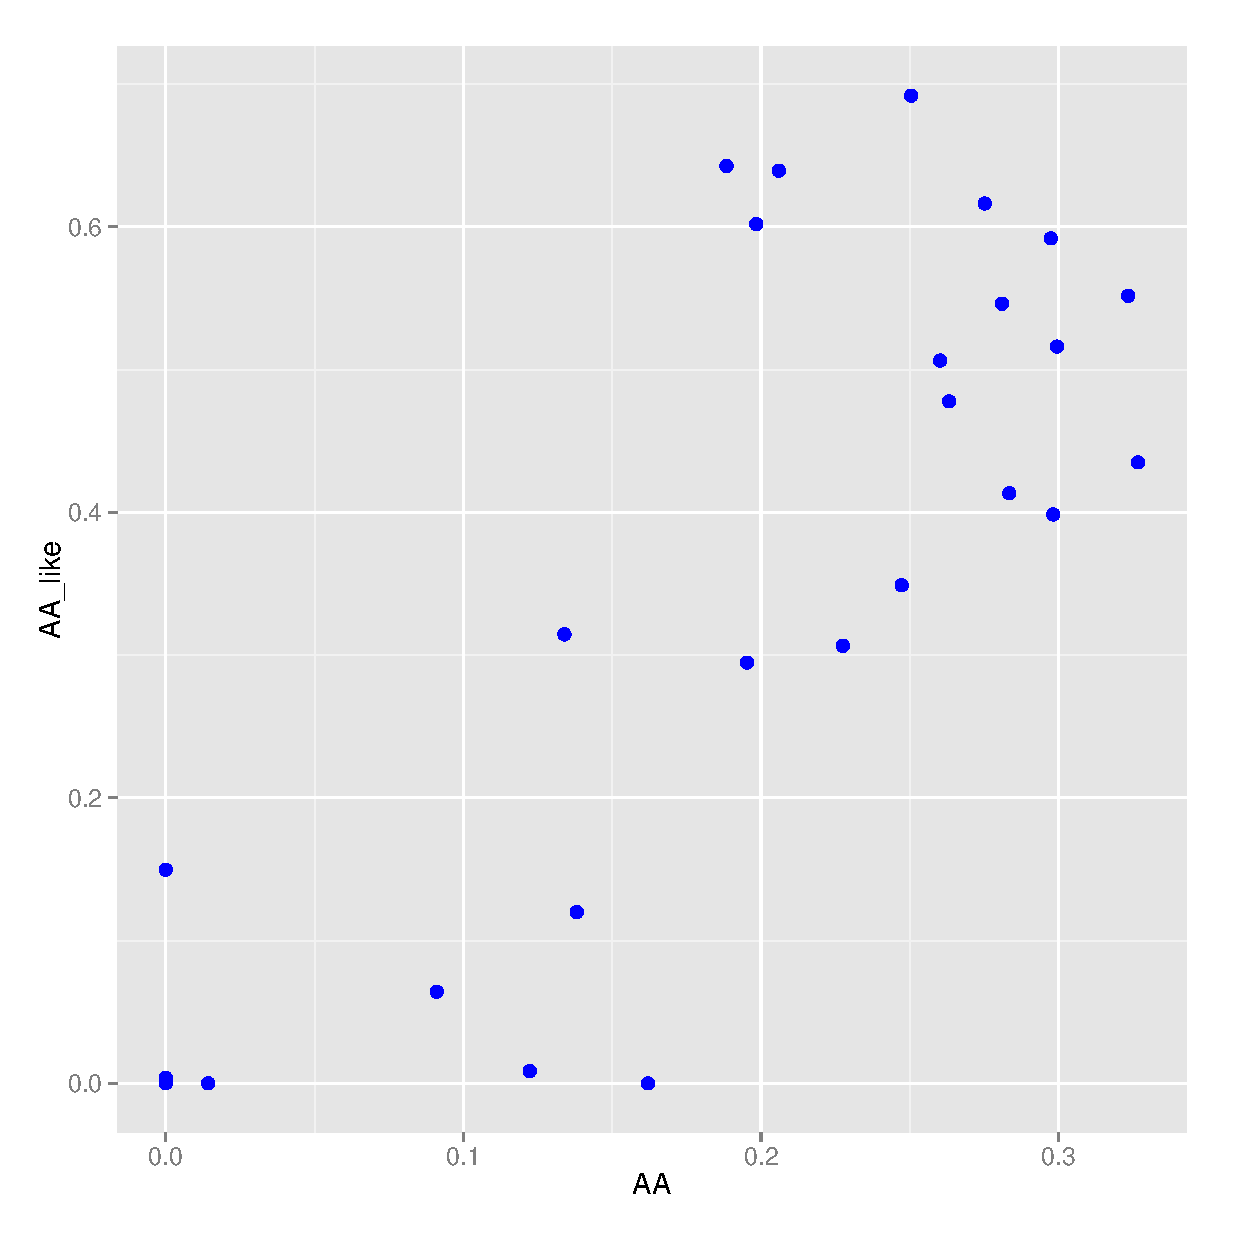
\includegraphics[width=10cm,height=10cm]{UTUC_AA_AAlike_cor.eps}
\caption{}
\label{example_signature.pd}
\end{figure}


\clearpage


% \begin{figure}
% \centering
% \includegraphics[width=15cm,height=15cm]{sig2_group.eps}
% \caption{Mutation signatures obtained for several cancer types categorized as Signature 2}
% \label{example_summary.pd}
% \end{figure}

% \clearpage

% \begin{figure}
% \centering
% \includegraphics[width=15cm,height=3.5cm]{sig6_group.eps}
% \caption{Mutation signatures obtained for several cancer types categorized as Signature 6}
% \label{example_summary.pd}
% \end{figure}

% \clearpage

% \begin{figure}
% \centering
% \includegraphics[width=15cm,height=3.5cm]{sig7_group.eps}
% \caption{Mutation signatures obtained for several cancer types categorized as Signature 7}
% \label{example_summary.pd}
% \end{figure}

% \clearpage

% \begin{figure}
% \centering
% \includegraphics[width=15cm,height=3.5cm]{sig19_group.eps}
% \caption{Mutation signatures obtained for several cancer types categorized as Signature 19}
% \label{example_summary.pd}
% \end{figure}


\end{document}

